\chapter{Mixture Distributions and Hidden Markov Models} 
\label{chap:mix}

Mixture distributions pop up in lots of places in probabilistic
modeling, so we devote a chapter to them here.  They also set the stage
for Hidden Markov Models, the other topic in this chapter.

\section{Two Motivating Examples}

\subsection{The Old Trick Coin Example, Updated}
\label{oldtrick}

Recall the trick coin example in Section \ref{caution}.  Let's look at a
somewhat different version.

Suppose we have a large box of coins of two types. One type has
probability $p_1$ of heads, the other probability $p_2$ of heads. A
proportion r of the coins is of the first type. We reach into the box,
choose a coin at random, and toss that coin 10 times, resulting in N
heads. What is the distribution of N?

Since $N$ is discrete, the distribution is described by its pmf, which is

\begin{equation}
\label{mixbinom}
p_N(k) = r \binom{10}{k} p_1^k (1-p_1)^{10-k} +
(1-r) \binom{10}{k} p_2^k (1-p_2)^{10-k}
\end{equation}

You can see why this is called a {\it mixture} model. The above pmf is a
mixture of two binomial pmfs, with mixing proportions r and 1-r.  

Let $C$ denote the type of coin we choose, 1 or 2, with heads
probabilities $p_1$ and $p_2$, respectively.  $P(C = 1) = r$ and
$P(C = 2) = 1-r$.  Conditioned on $C$, the random variable $N$
is binomial with success probabilities $p_1$ or $p_2$, depending on $C$;
more succinctly, the conditional distribution of $N$, given $C$,
is binomial with success probability $p_C$.  (The number of trials is
10.)

\subsection{Old Faithful Geyser}

The dataset here is included in R, under the name \textbf{faithful}.  It
is collected from the famous geyser in Yellowstone National Park in the
US, named Old Faithful.  The call

\begin{lstlisting}
hist(faithful$waiting)
\end{lstlisting}

requesting a histogram of the intereruption times,
yields Figure \ref{faithfulhist}.

\begin{figure}[tb]
\centerline{
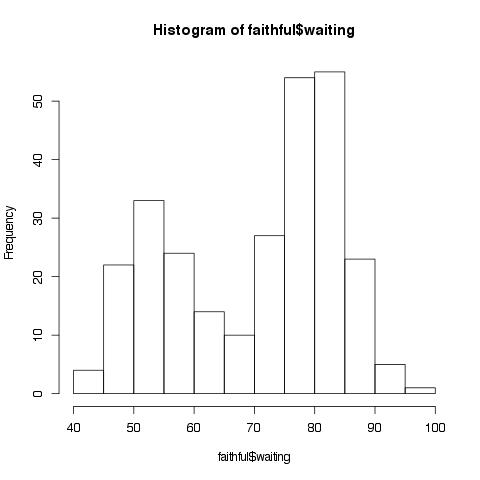
\includegraphics[width=3.0in]{Faithful.jpg}
}
\caption{Old Faithful waiting times}
\label{faithfulhist}
\end{figure}

It looks like two normal distributions may be at work down there
underground, resulting in different kinds of eruptions.  Let $T$
denote the type of eruption, 1 or 2, with probabilities $s$ and $1-s$.
We may wish to model the waiting time between eruptions that we see
above ground, $W$, as normally distribted with mean $\mu_1$ or $\mu_2$,
depending on $T$  The $\mu_i$ would be parameters, along with the
corresponing variances, and the mixing proportion $s$.

We will see later that Hidden Markov Models also consist of
latent---hidden---variables and observed ones.  The latent variables
are states of a Markov chain.

Note that the latent variable could be unobserved but physical, e.g. the
choice of the coin, or merely postulated, as with the two-process model
we surmise for the geyser.

\section{The Notion of ``Latent'' Variables}

The word \textit{latent} in general usage means ``unseen,'' which is
essentially its statistical meaning.  In the coin example, $C$ is
latent, as we cannot visually tell what type of coin it is.  In the
geyser example, $T$ is truly unseen, underground.  By contrast, $N$
in the coin example and $W$ for the geyser are definitely observed.jj

\section{General Mixture Distributions}
\label{genmix}

\subsection{Notation}

First, recall the general convention that for any random variable $Y$,
its probability mass function is denoted by $p_Y$ if $Y$ is discrete,
and its density is denoted by $f_Y$ in the continuous case.  Its cdf is
$F_Y$, in any case, discrete, continuous or mixed.

Notation for conditional distribution is similar, but note that now
these functions will have two arguments instead of one.  For example,

\begin{equation}
p_{V | U}(i,j) = P(V = j | U = i)
\end{equation}

Now back in the specific context of mixture distribution,
let $M$ denote the mixing variable, e.g. $C$ and $T$ above, and let $X$
be the ``mixee,'' the variable being mixed according to the value of
$M$.  The conditional distribution of $X$ depends on $M$.  

\subsection{Definition}

It's easiest to define the concept of $X$ having a mixing distribution 
by just consider some cases:

\begin{itemize}

\item $M$ discrete, $X$ discrete:  

\begin{equation}
\label{mdscxdisc}
p_X(i) = \sum_j p_{X|M} (i,j) ~ p_M(j)
\end{equation}

\item $M$ continuous, $X$ continuous:  

\begin{equation}
\label{mcontinxcontin}
f_X(t) = \int_{s \in A} f_{X|M}(t,s) ~  f_M(s) ~ ds
\end{equation}

\end{itemize}

The reader can fill in other cases.  For instance, in the geyser
example, $X$ would be continuous but $M$ discrete.

Actually, the definition isn't so abstract after all.  Equation
(\ref{mdscxdisc}) should look quite familiiar, with the reader having
encountered this form many times in earlier courses.  Equation
(\ref{mcontinxcontin}) is probably less familiar, but it is a direct
analog of (\ref{mdscxdisc}).

In other words, the distribution of $X$, say in the discrete/discrete case,
is a weighted average of the condiitonal distribution of $X$, with the
weights being the pmf of $M$.  Note that this implies that the weights
most be nonnegative and sum to 1.\footnote{Some readers may recognize
this as a {\bf convex combination}.}  In the case of $M$ continuous, the
weights are nonnegative and integrate to 1.

Mixture distributions occur in a surprisingly wide variety of
applications, and thus this material should be mastered.  It is somewhat
difficult at first, but if you always keep concrete examples such as the
trick coin problem in mind, it is not bad at all.

By the way, there is nothing in the above definition that limits the
$G_i$ and H to be for scalar random variables.  They could all be
bivariate, for instance (though of course they all have to be of the
same dimension.)

\section{Generating Random Variates from a Mixture Distribution}

One way to get additional insight on mixture distributions is to think
about how to simulate them.  For instance, consider the trick coin problem.
The following R code simulates $X_i$:

\begin{lstlisting}
rxi <- function(i) {
   m <- sample(0:1,1)
   p <- if (M ==0) 0.1 else 0.9
   rbinom(1,i,p)
}
\end{lstlisting}

In general:

\begin{itemize}

\item We first generate M.

\item Then we generate a random variable from the pmf $G_M$.

\end{itemize}

Various examples of mixture distributions will be presented in this
chapter.  But first, we need to develop some machinery.

% \section{Conditional Distributions}
% 
% The key to good probability modeling and statistical analysis is to
% understand conditional probability.  The issue arises constantly.
% 
% \subsection{Conditional Pmfs and Densities}
% 
% First, let's review:  In many repetitions of our ``experiment,'' P(A) 
% is the long-run proportion of the time that A occurs.  By contrast,
% P(A$|$B) is the long-run proportion of the time that A occurs, {\it
% among those repetitions in which B occurs.}  Keep this in your mind at
% all times.
% 
% Now we apply this to pmfs, densities, etc.  We define the conditional
% pmf as follows for discrete random variables X and Y:
% 
% \begin{equation}
% \label{discrcond}
% p_{Y|X}(j|i) = P(Y = j | X = i) = \frac{p_{X,Y}(i,j)}{p_X(i)}
% \end{equation}
% 
% By analogy, we define the conditional density for continuous X and Y:
% 
% \begin{equation}
% \label{contcond}
% f_{Y|X}(t|s) = \frac{f_{X,Y}(s,t)}{f_X(s)}
% \end{equation}
% 
% \subsection{Conditional Expectation}
% 
% Conditional expectations are defined as straightforward extensions of
% (\ref{discrcond}) and (\ref{contcond}):
% 
% \begin{equation}
% E(Y|X=i) = \sum_{j} j p_{Y|X}(j|i) 
% \end{equation}
% 
% \begin{equation}
% E(Y | X = s) = \int_{t} t f_{Y|X}(t|s) ~ dt
% \end{equation}

\section{Review: the Laws of Total Expectation and Variance}
\label{lte}

Since mixture models involve conditional distributions, it should be no
surprise that the famous equations come into play.  First, the Law  of
Total Expectation

\begin{equation}
\label{itex}
E(Y)=E[E(Y|W)]
\end{equation}

for any random variables Y and W (for which the expectations are
defined).  

The RHS of (\ref{itex}) looks odd at first, but it's merely E[g(W)];
since Q =  E(Y$|$W) is a random variable, we can certainly ask what its
expected value is.

And the Law of Total Variance,

\begin{equation}
\label{bis}
Var(Y)=E[Var(Y|W)]+Var[E(Y|W)]
\end{equation}

Note that the RHSs of (\ref{hsum}) and (\ref{continmix}) can be written as

\begin{equation}
E[ P(M = k | G) ]
\end{equation}

and

\begin{equation}
E[ E(f_M (G) | G)]
\end{equation}

where $G$ is the mixing variable.  And in both cases

\begin{equation}
\label{generalmix}
F_M(t) = E[ P(M \leq t ) | G) ]
\end{equation}

Actually, (\ref{generalmix}) is the only fully general to state a
mixture distribution.  For any random variable $X$, its distribution is
completely characterized by $F_x$.  So, (\ref{generalmix}) defines the
mixing relation fully, and for any distribution for $G$ and $M$, whether
discrete, continuous or mixed.


\section{Estimation by Method of Maximum Likelihood and the Method of
Moments}

We wlll need to be able to estimate parameters from data.  Here we
briefly cover the two most famous methods for this.

To see how MLE works, consider the following game.  I toss a coin until
I accumulate $r$ heads.  I don't tell you what value I've chosen for
$r$, but I do tell you $K$, the number of tosses I needed.  You then
must guess the value of $r$.  Well, $K$ has a negative binomial
distribution (Section \ref{negbin}), so

\begin{equation}
P(K = u) = \binom{u-1}{r-1} 0.5^u,~ u = r, r+1, ...
\end{equation} 

Say I tell you $K = 7$.  Then what you might do is find the value of $r$
that maximizes

\begin{equation}
\label{negbin7}
\binom{6}{r-1} 0.5^7
\end{equation}

You are asking, ``What value of $r$ would have made our data ($K = 7$)
most likely?''  Trying $r = 1,2,...,7$, one finds that $r = 4$ maximizes
(\ref{negbin7}), so we would take that as our guess.

For a random variable $X$, the number $E(X^k)$ is called the $k^{th}$
\textit{moment} of $X$.  The Method of Moments approach works by
matching estimated moments of our data to the sample moments.

For the negative binomial distribution it is known that $E(K) = r/p$,
where $p$ is the probability of ``success,'' in this setting meaning
heads.  So $E(K) = 2r$.  Under MM, we would set $\overline{K} = 2
\widehat{r}$, where the left-hand side is the average of all values of
$K$ in our data.  We only did the ``experiment'' once, say in this case
with $K = 6$, so $\overline{K} = 6$ and we guess $r$ to be 3.

\section{The EM Algorithm}
\label{emalg}

Now returning to our main topic of mixture models, let's discuss a very
common tool for fitting such models, the EM (Expectation-Maximization)
Algorithm.  

\subsection{Overall Idea}

EM works in an iterative manner, in alternating cycles.  Consider again
the trick coin example.  We want to both estimate the parameters $p$,
$q$ and $r$, and also want to guess the value(s) of our latent variable,
$C$.  Why the plural in referring to $C$?  It could be that we perform
the above experiment, say, 50 times, resulting in our data
$N_1,...,N_{50}$, and our latent values $C_1,...C_{50}$.  
Say we know $r$, to make this explanation simpler.

EM then works as follows:  We first make initial guesses for $p_1$ and $p_2$
and $r$, and the alternate the following two actions:

\begin{itemize}

\item[(a)] Guess the values of the $C_i$, based on our current guesses for
the parameters and the $N_i$.

\item[(b)] Generate new guesses for the values of the parameters, based on
our current guesses for the latent variables and the $N_i$.

\item Then back to step (a) etc.

\end{itemize} 

Hopefully the process converges!

The guesses are typcally MLEs.  Let's look at this in a bit more detail.
Say we perform the coin experiment just once, for simplicity.  Then our
observed datum $N$ has, as noted, a binomial distribution with 10 trials
and success probability $p_C$, $C = 1,2$.  The likelihood is

\begin{equation}
\label{binlikeA}
\binom{10}{N} p_C^N (1-p_C)^{10-N}
\end{equation}

Remember, $N$ is known, and $p_1$ and $p_2$ are considered known (in all
step (a)s).  So, our MLE of $C$ is whichever value of $C$, 1 or 2, makes
(\ref{binlikeA}) larger.  If we have collected 50 sample observations, we
estimate the $C_i$ is the same way.

Then in step (b), the likelihood is

\begin{equation}
\label{binlikeB}
\Pi_{i=1}^n
\left [ \binom{10}{N_i} p_{C_i}^{N_i} (1-p_{C_i})^{10-N_i} 
\right ]
\end{equation}

Now the tables have turned.  The $C_i$ are assumed known (for the time
being), but $p_1$ and $p_2$ are unknown.  We estimate them using MLE,
maximizing (\ref{binlikeB}).

After taking derivatives, etc., one would end up with a messy, nonlinear
set of equations to solve.  One could try R's {\bf mle()} function, but
even that may be rather complex.  Fortunately, R libraries exist, such
as {\bf mixtools}, so you can avoid knowing all the details, as long as
you understand the basic notion of a mixture model and the overall plan
for EM.  

\subsection{The mixtools Package}

R's CRAN repository of contributed software includes the {\bf mixtools}
library.  Let's see how to use one of the functions in that library,
{\bf normalmixEM()}, which assumes that the densities in
(\ref{continmix}) are from the normal distribution family.

Let's suppose we are modeling the data as a mixture of 2 normals.
So, with our observed data set, our goal is to estimate 5 parameters
from our data:  

\begin{itemize}

\item $\mu_1$, the mean of the first normal distribution 

\item $\mu_2$, the mean of the second normal distribution 

\item $\sigma_1$, the mean of the second normal distribution 

\item $\sigma_2$, the mean of the second normal distribution 

\item q = P(M = 1) = 1 - P(M = 2)

\end{itemize}

The basic form of the call is 

\begin{lstlisting}
normalmixEM(x,lambda=NULL,mu=NULL,sigma=NULL,k=2)
\end{lstlisting}

where

\begin{itemize}

\item {\bf x} is the data, a vector

\item {\bf lambda} is a vector of our initial guesses for the quantities
P(M = i), of length {\bf k} (recycling will be used if it is shorter);
note that these must be probabilities summing to 1

\item {\bf mu} is a vector of our initial guesses for the $\mu_i$

\item {\bf sigma} is a vector of our initial guesses for the $\sigma_i$

\item {\bf k} is the number of values M can take on, e.g. 2 for a
mixture of 2 normals

\end{itemize}

One can leave the initial guesses as the default NULL values, but
reasonable guesses may help convergence.

The return value will be an R list, whose components include {\bf
lambda}, {\bf mu} and {\bf sigma}, the final estimates of those values.

\subsection{Example:  Old Faithful Geyser}

This example is taken from the online documentation in {\bf mixtools}.
The data concern the Old Faithful Geyser, a built-in data set in R.

The data here consist of waiting times between eruptions.  A histogram,
obtained via 

\begin{lstlisting}
> hist(faithful$waiting)
\end{lstlisting}

and shown in Figure \ref{faithfulhist}, seems to suggest that the
waiting time distribution is a mixture of 2 normals. 

I tried initial guesses of means and standard deviations from the
appearance of the histogram, and used equal weights for my initial
guesses in that aspect:

\begin{lstlisting}
> mixout <- normalmixEM(faithful$waiting,lambda=0.5,mu=c(55,80),sigma=10,k=2)
number of iterations= 9 
> str(mixout)
List of 9
 $ x         : num [1:272] 79 54 74 62 85 55 88 85 51 85 ...
 $ lambda    : num [1:2] 0.361 0.639
 $ mu        : num [1:2] 54.6 80.1
 $ sigma     : num [1:2] 5.87 5.87
 $ loglik    : num -1034
 $ posterior : num [1:272, 1:2] 1.02e-04 1.00 4.12e-03 9.67e-01 1.21e-06
...
  ..- attr(*, "dimnames")=List of 2
  .. ..$ : NULL
  .. ..$ : chr [1:2] "comp.1" "comp.2"
 $ all.loglik: num [1:10] -1085 -1051 -1037 -1034 -1034 ...
 $ restarts  : num 0
 $ ft        : chr "normalmixEM"
 - attr(*, "class")= chr "mixEM"
\end{lstlisting}

So, the estimate from EM is that about 36\% of the eruptions are of Type
1, etc.  Interesting, when I tried it without my own initial guesses,

\begin{lstlisting}
mixout <- normalmixEM(faithful$waiting,k=2)
\end{lstlisting}

the results were the same, so it seems to be a fairly stable model here.

By the way, since we are working with a hidden variable M here---in
fact, we are merely postulating that it exists---how do we check this
assumption?  We'll return to this general idea of model fitting in
Chapter \ref{chap:mod}.

\section{Mean and Variance of Random Variables Having Mixture
Distributions}
\label{mixmeanvar}

Think of the random variables M and Y in the discussion following
(\ref{continmix}).  Then EY is easy to find using the Law of Total
Expectation:

\begin{equation}
\label{mixmean}
EY = E[E(Y | M)]
\end{equation}

Of course, evaluating this would require being able to compute E(Y $|$
M), which is easy in some cases, not so easy in others.

Also, using the Law of Total Variance, we have that

\begin{equation}
\label{mixvar}
Var(Y) = E[Var(Y|M)] + Var[E(Y|M)]
\end{equation}

\section{Example:  Two Kinds of Batteries}

Say a factory produces two kinds of batteries.  One kind has lifetime
that is exponentially distributed with mean 200 and the other's
distribution is exponential with mean 500.  Suppose 60\% of the
factory's production is of the former type, with 40\% being of the
latter type.  Let's find the mean and variance of the lifetime Y of a
randomly chosen battery.

Note that the distribution of Y is a mixture, in the sense of Section
\ref{genmix}, in particular (\ref{continmix}).  Y here is a continuous
random variable, referred to in that section as the ``continuous
outcome'' case.   In the notation there, let M be the battery type, with
M being 0 or 1, for the 200-hour and 500-hour batteries, respectively.
The conditional density of Y given M = 0 is exponential with mean 200,
while given M = 1 it is exponential with mean 500.  The unconditional
density of Y is the mixture of these two exponential densities, as 
(\ref{continmix}).

We want to find the \underline{un}conditional mean and variance of Y.

Then

\begin{equation}
\label{batt1}
E(Y|M)=\left\{ \begin{array}{rl}
200, & w.p. ~ 0.60 \\
500, & w.p. ~ 0.40
\end{array}\right. 
\end{equation}

and 

\begin{equation}
\label{batt2}
Var(Y|M)=\left\{ \begin{array}{rl}
200^2, & w.p. ~ 0.60 \\
500^2, & w.p. ~ 0.40
\end{array}\right. 
\end{equation}

(recalling that in the exponential family, variance is the square of the
mean).

We can now use the formulas in Section \ref{mixmeanvar}.  Let $Q_1 =
E(Y|M)$  and $Q_2 = Var(Y|M)$.  Then

\begin{equation}
EY = EQ_1 = 0.60 \times 200 + 0.40 \times 500
\end{equation}

and 

\begin{eqnarray}
Var(Y) &=& E(Q_2) + Var(Q_1) \\
&=& (0.60 \times 200^2 + 0.40 \times 500^2) + Var(Q_1) \\
&=& (0.60 \times 200^2 + 0.40 \times 500^2) + E(Q_1^2) - (EQ_1)^2 \\
&=& (0.60 \times 200^2 + 0.40 \times 500^2) + (0.60 \times 200^2 + 0.40
\times 500^2)  \\
& & - (0.60 \times 200 + 0.40 \times 500)^2 \\
\end{eqnarray}

\section{Example:  Overdispersion Models}

A common model used in practice is that of {\bf overdispersion}, in
connection with Poisson models.  

Recall the following about the Poisson distribution family:

\begin{itemize}

\item [(a)] This family is often used to model counts.

\item [(b)] For any Poisson distribution, the variance equals the mean.

\end{itemize}

In some cases in which we are modeling count data, condition (b) is too
constraining.  We want a ``Poisson-ish''
distribution in which the variance is greater
than the mean, called {\bf overdispersion}.  

One may then try to fit a mixture of several Poisson distributions,
instead of a single one.  This does induce overdispersion, as we will
now see.  

Suppose M can equal 1,2,...,k, with probabilities $p_1,...,p_k$ that sum
to 1.  Say the distribution of Y given M = i is Poisson with parameter
$\lambda_i$.  Then Y has a mixture distribution.  Our goal here will be
to show that Y is overdispersed, i.e. has a large variance than mean.

By the Law of Total Expectation,

\begin{eqnarray}
\label{meanlamb}
EY &=& E[E(Y|M)] \\ 
&=& E(\lambda_M) \label{elambm} \\
&=& \sum_{i=1}^k p_i \lambda_i
\end{eqnarray}

Note that in the above, the expression $\lambda_M$ is a random variable,
since its subscript M is random.  Indeed, it is a function of M, so
Equation (\ref{egofx}) then applies, yielding the final equation.  The
random variable $\lambda_M$ takes on the values $\lambda_1,...,\lambda_k$
with probabilities $p_1,...,p_k$, hence that final sum.

The corresponding formula for variance, (\ref{bis}), can be used to
derive Var(Y).

\begin{eqnarray}
Var(Y) &=& E[Var(Y|M)] + Var[E(Y|M)] \\ 
&=& E(\lambda_M) + Var(\lambda_M) \label{thislast} \\
&=& EY + Var(\lambda_M) \label{thislast} \\
\end{eqnarray}

Did you notice that this last equation achieves our goal of showing
overdispersed?  Since

\begin{equation}
Var(\lambda_M) > 0
\end{equation}

we have that

\begin{equation}
Var(Y) > E(\lambda_M) = EY
\end{equation}

by (\ref{elambm}).

But let's see just how much greater the variance is than the mean.  The
second term in (\ref{thislast}) is evaluated the same way as in
(\ref{elambm}):  This is the variance of a random variable that takes on
the values $\lambda_1,...,\lambda_k$ with probabilities $p_1,...,p_k$,
which is

\begin{equation}
\sum_{i=1}^k p_i (\lambda_i - \overline{\lambda})^2
\end{equation}

where 

\begin{equation}
\overline{\lambda} =  E\lambda_M = \sum_{i=1}^k p_i \lambda_i
\end{equation}

Thus

\begin{equation}
EY = \overline{\lambda}
\end{equation}

and

\begin{equation}
Var(Y) = \overline{\lambda} + 
\sum_{i=1}^k p_i (\lambda_i - \overline{\lambda})^2
\end{equation}

So, as long as the $\lambda_i$ are not equal, we have

\begin{equation}
Var(Y) > EY
\end{equation}

in this Poisson mixture model, in contrast to the single-Poisson case
in which Var(Y) = EY.  You can now see why the Poisson mixture model is
called an overdispersion model.

So, if one has count data in which the variance is greater than the
mean, one might try using this model.

In mixing the Poissons, there is no need to restrict to discrete M.  In
fact, it is not hard to derive the fact that if X has a gamma
distribution with parameters r and p/(1-p) for some $0 < p < 1$, and Y
given X has a Poisson distribution with mean X, then the resulting Y
neatly turns out to have a negative binomial distribution.

\section{Example:  Hidden Markov Models}

The Hidden Markov Model to be introduced in Section \ref{hmm} fits our
definition of a mixture distribution, with M being the mixing variable.

According, the machinery of mixing models applies.  For instance, we can
use the EM algorithm to calculate various quantities.

% \section{Example:  Cluster Analysis}
% 
% We will in Section \ref{mixclust} see that the notion of mixtures can
% also be applied to clustering.
% 
% \section{Markov Chain with Random $X_0$}
% 
% LOSE MARKOV PROPERTY
% 
% \section{Bayes Models, Including Empiricial Bayes}
% 
% JUST REFER TO THE BAYES SECTION, BUT NOTE IN THE LATTER THAT IT IS A
% MIXTURE

% \section{De Finetti's Theorem}
% 
% Consider again the trick coin example, Section \ref{oldtrick}.  As we
% have discussed, the tosses $B_i$ are not independent.  However, they are
% {\bf exchangeable}:
% 
% \begin{equation}
% P(B_
% \end{equation}


\section{Vector Space Interpretations (for the mathematically
adventurous only)}
\label{adventure}

The abstract vector space notion in linear algebra has many applications
to statistics.  We develop some of that material in this section.

% Consider the set of all random variables associated with some
% ``experiment,'' in our ``notebook'' sense from Section \ref{repeatexpt}.
% (In more mathematical treatments, we would refer here to the set of all
% random variables defined on some {\bf probability space}.)  Note that
% some of these random variables are independent of each other, while
% others are not; we are simply considering the totality of all random
% variables that arise from our experiment.

Let $\cal V$ be the set of all such random variables having finite
variance and mean 0.  We can set up $\cal V$ as a vector space.  For that,
we need to define a sum and a scalar product.  Define the sum of any two
vectors X and Y to be the random variable X+Y.  For any constant c, the
vector cX is the random variable cX.  Note that $\cal V$ is closed under
these operations, as it must be:  If X and Y both have mean 0, then X+Y
does too, and so on.

Define an inner product on this space:

\begin{equation}
(X,Y) = Cov(X,Y) = E(XY) 
\end{equation}

(Recall that Cov(X,Y) = E(XY) - EX EY, and that we are working with
random variables that have mean 0.) Thus the norm of a vector X is

\begin{equation}
||X|| = {(X,X)}^{0.5} = \sqrt{E(X^2)} = \sqrt{Var(X)}
\end{equation}

again since E(X) = 0.

\subsection{Properties of Correlation}
\label{propcorr}

The famous Cauchy-Schwarz Inequality for inner products says,

\begin{equation}
|(X,Y)| \leq ||X|| ~ ||Y||
\end{equation}

Applying that here, we have

\begin{equation}
|\rho(X,Y)| \leq 1
\end{equation}

So, vector space theory tells us that correlations are bounded between
-1 and 1.

Also, the Cauchy-Schwarz Inequality yields equality if and only if one
vector is a scalar multiple of the other, i.e. Y = cX for some c.
When we then translate this to random variables of nonzero means,
we get Y = cX + d.  

In other words, the correlation between two random variables is between
-1 and 1, with equality if and only if one is an exact linear function
of the other.

\subsection{Conditional Expectation As a Projection}
\label{elegant} 

For a random variable X in $\cal V$, let $\cal W$ denote the subspace of
$\cal V$ consisting of all functions h(X) with mean 0 and finite
variance.  (Again, note that this subspace is indeed closed under vector
addition and scalar multiplication.) 

Now consider any Y in $\cal V$.  Recall that the {\it projection} of Y
onto $\cal W$ is the closest vector T in $\cal W$ to Y, i.e. T minimizes
$||Y-T||$.  That latter quantity is 

\begin{equation}
\label{l2}
{\left ( E[{(Y-T)}^2] \right )}^{0.5}
\end{equation}

To find the minimizing T, consider first the minimization of

\begin{equation}
\label{minsc}
E[{(S-c)}^2]
\end{equation}

with respect to constant c for some random variable S.  We already
solved this problem back in Section \ref{gofc}.  The minimizing value 
is c = ES.

Getting back to (\ref{l2}), use the Law of Total Expectation to write

\begin{equation}
\label{min2}
E[{(Y-T)}^2] = E \left (  E[{(Y-T)}^2|X]\right )
\end{equation}

From what we learned with (\ref{minsc}), applied to the conditional
(i.e. inner) expectation in (\ref{min2}), we see that the T which
minimizes (\ref{min2}) is T = E(Y$|$X).  

In other words, the conditional mean is a projection!  Nice, but is this
useful in any way?  The answer is yes, in the sense that it guides the
intuition.  All this is related to issues of statistical
prediction---here we would be predicting Y from X---and the geometry
here can really guide our insight.  This is not very evident without
getting deeply into the prediction issue, but let's explore some of the
implications of the geometry.

For example, a projection is perpendicular to the line connecting the
projection to the original vector.  So

\begin{equation}
\label{err}
0 = (E(Y|X),Y-E(Y|X)) 
% = E \left [ E(Y|X) \left ( Y-E(Y|X) \right ) \right ]
= Cov[E(Y|X), ~ Y-E(Y|X)]
\end{equation}

This says that the prediction E(Y$|$X) is uncorrelated with the
prediction error, Y-E(Y$|X$).  This in turn has statistical importance.
Of course, (\ref{err}) could have been derived directly, but the
geometry of the vector space intepretation is what suggested we look at
the quantity in the first place.  Again, the point is that the vector
space view can guide our intuition.

Simlarly, the Pythagorean Theorem holds, so

\begin{equation}
\label{py}
{||Y||}^2 = {||E(Y|X)||}^2 + {||Y-E(Y|X)||}^2
\end{equation}

which means that

\begin{equation}
\label{py2}
Var(Y) = Var[E(Y|X)] + Var[Y-E(Y|X)]
\end{equation}

Equation (\ref{py2}) is a common theme in linear models in statistics,
the decomposition of variance.  

There is an equivalent form that is useful as well, derived as follows
from the second term in (\ref{py2}).  Since

\begin{equation}
E[Y-E(Y|X)] = EY - E[E(Y|X)] = EY - EY = 0
\end{equation}

we have

\begin{eqnarray}
\label{verycomplex}
Var[Y-E(Y|X)] &=& E \left [ (Y-E(Y|X))^2 \right ] \\ 
&=& E \left [ Y^2 -2YE(Y|X) + (E(Y|X))^2 \right ] 
\end{eqnarray}

Now consider the middle term, $E[-2YE(Y|X)]$.  Conditioning on X and
using the Law of Total Expectation, we have

\begin{equation}
E[-2YE(Y|X)] = -2 E \left [ (E(Y|X))^2 \right ]
\end{equation}

Then (\ref{verycomplex}) becomes

\begin{eqnarray}
Var[Y-E(Y|X)] &=& E (Y^2) - E \left [ (E(Y|X))^2 \right ] \\
&=& E \left [ E(Y^2 | X) \right ] - E \left [ (E(Y|X))^2 \right ] \\
&=& E \left ( E(Y^2 | X) - (E(Y|X))^2 \right ) \\
&=& E \left [ Var(Y|X) \right ]
\end{eqnarray}

the latter coming from our old friend, $Var(U) = E(U^2) - (EU)^2$, with
U being Y here, under conditioning by X.

In other words, we have just derived another famous formula:

\begin{equation}
Var(Y) = E[Var(Y|X)] + Var[E(Y|X)]
\end{equation}

\section{Proof of the Law of Total Expectation}
\label{proveitex} 

Let's prove (\ref{itex}) for the case in which W and Y take values only
in the set \{1,2,3,...\}.  Recall that if T is an integer-value random
variable and we have some function h(), then L = h(T) is another random
variable, and its expected value can be calculated as\footnote{This is
sometimes called The Law of the Unconscious Statistician, by nasty
probability theorists who look down on statisticians.  Their point is
that technically $EL = \sum_k k P(L = k)$, and that (\ref{unconscious})
must be proven, whereas the statisticians supposedly think it's a
definition.}  

\begin{equation}
\label{unconscious}
E(L) = \sum_k h(k) P(T = k)
\end{equation}

In our case here, Q is a function of W, so we find its expectation from
the distribution of W:

\begin{eqnarray*}
E(Q) & = & \sum ^{\infty }_{i=1}g(i) P(W=i)\\
 & = & \sum ^{\infty }_{i=1}E(Y|W=i)P(W=i)\\
 & = & \sum ^{\infty }_{i=1} \left [ \sum ^{\infty }_{j=1}jP(Y=j|W=i) \right ] P(W=i) \\
 & = & \sum ^{\infty }_{j=1}j\sum ^{\infty }_{i=1}P(Y=j|W=i)P(W=i)\\
 & = & \sum ^{\infty }_{j=1}jP(Y=j)\\
 & = & E(Y)
\end{eqnarray*}
 In other words, 

\begin{equation}
E(Y)=E[E(Y|W)]
\end{equation}

\startproblemset

\oneproblem
In the catchup game in Section \ref{catchupgame}, let $V$ and $W$ denote
the winnings of the two players after only one turn.  Find $P(V > 0.4)$.

\oneproblem 
Suppose one keeps rolling a die. Let $S_n$ denote the total
number of dots after n rolls, mod 8, and let $T$ be the number of rolls
needed for the event $S_n = 0$ to occur. Find $E(T)$, using an approach
like that in the ``trapped miner'' example in Section
\ref{trappedminer}.

\oneproblem
In our ordinary coins which we use every day, each one has a slightly 
different probability of heads, which we'll call $H$.  Say $H$ has 
the distribution $N(0.5, 0.03^2)$.  We choose a coin from a batch at 
random, then toss it 10 times.  Let $N$ be the number of heads we get.  
Find $Var(N)$.

\oneproblem
Suppose the number N of bugs in a certain number of lines of code has a
Poisson distribution, with parameter L, where L varies from one
programmer to another. Show that Var(N) = EL + Var(L).

\oneproblem
This problem arises from the analysis of random graphs, which for
concreteness we will treat here as social networks such as Facebook.

In the model here, each vertex in the graph has N friends, N being a
random variable with the same distribution at every vertex. One thinks
of each vertex as generating its links, unterminated, i.e. not tied yet
to a second vertex. Then the unterminated links of a vertex pair off at
random with those of other vertices. (Those that fail will just pair in
self loops, but we'll ignore that.)

Let M denote the number of friends a friend of mine has. That is, start
at a vertex A, and follow a link from A to another vertex, say B. M is
the number of friends B has (we'll include A in this number).

\begin{itemize}

\item [(a)] Since an unterminated link from A is more likely to pair up
with a vertex that has a lot of links, a key assumption is that P(M = k)
= ck P(N = k) for some constant c. Fill in the blank: This is an example
of the setting we studied called \_\_\_\_\_\_\_\_\_\_\_\_\_\_\_\_\_.

\item [(b)] Show the following relation of generating functions: $g_M(s)
= g_N'(s)/EN$. 

\end{itemize}

\oneproblem
Suppose Type 1 batteries have exponentially distributed lifetimes with
mean 2.0 hours, while Type 2 battery lifetimes are exponentially
distributed with mean 1.5.  We have a large box containing a mixture of
the two types of batteries, in proportions q and 1-q.  We reach into the
box, choose a battery at random, then use it.  Let $Y$ be the lifetime
of the battery we choose.  Use the Law of Total Variance, (\ref{bis}),
to find $Var(Y)$.


\oneproblem
In the backup battery example in Section \ref{backup}, find Var(W),
using the Law of Total Expectation.

\oneproblem
Let X denote the number we obtain when we roll a single die
once.  Let $G_X(s)$ denote the generating function of X.

\begin{itemize}

\item [(a)] Find $G_X(s)$.

\item [(b)] Suppose we roll the die 5 times, and let T denote the
total number of dots we get from the 5 rolls.  Find $G_T(s)$.

\end{itemize}

\oneproblem
Consider this model of disk seeks. For simplicity, we'll assume a very
tiny number of tracks, 3. Let $X_1$ and $X_2$ denote the track numbers
of two successive disk requests. Each has a uniform distribution on
\{1,2,3\}. But given $X_1 = i$, then $X_2 = i$ with probability 0.4, with
$X_2$ being j with probability 0.3, $j \neq i$. (Convince yourself that
these last two sentences are consistent with each other.) Find the
following:

\begin{itemize}

\item [(a)] $P(|X_1 - X_2| \leq 1)$

\item [(b)] $E(|X_1 - X_2|)$

\item [(c)] $F_{X_1,X_2}(2,2)$

\end{itemize}

\oneproblem
Consider the computer worm example in Section \ref{senthi}.  Let R
denote the time it takes to go from state 1 to state 3.  Find $f_R(v)$.  
(Leave your answer in integral form.)

\oneproblem
Suppose (X,Y) has a bivariate normal distribution, with EX = EY = 0,
Var(X) = Var(Y) = 1, and $\rho(X,Y) = 0.2$.  Find the following, in
integral forms:

\begin{itemize}

\item [(a)] $E(X^2+XY^{0.5})$

\item [(b)] $P(Y > 0.5X)$

\item [(c)] $F_{X,Y}(0.6,0.2)$

\end{itemize}
                      
\oneproblem
Suppose $X_i$, i = 1,2,3,4,5 are independent and each have mean 0 and   
variance 1.  Let $Y_i = X_{i+1} - X_i$, i = 1,2,3,4.  Using the 
material in Section \ref{matrix}, find the covariance matrix of 
$Y = (Y_1, Y_2, Y_3, Y_4)$.

% Plot of 2-D normal, adapted from R Graph Gallery,
% http://addictedtor.free.fr/graphiques/graphcode.php?graph=42:
% 
% mu1 <- 0  # EX1
% mu2 <- 0  # EX2
% s11 <- 10  # Var(X1) = 10
% s22 <- 10  # Var(X2) = 15
% x1 <- seq(-10,10,length=41) 
% x2 <- x1 
% 
% # bivariate normal density
% f <- function(x1,x2,rho){
%         term1 <- 1/(2*pi*sqrt(s11*s22*(1-rho^2)))                               
%         term2 <- -1/(2*(1-rho^2))                                               
%         term3 <- (x1-mu1)^2/s11                                                 
%         term4 <- (x2-mu2)^2/s22                                                 
%         term5 <- 2*rho*((x1-mu1)*(x2-mu2))/(sqrt(s11)*sqrt(s22))               
%         term1*exp(term2*(term3+term4-term5))                                    
% } 
% 
% plot2dnorm <- function(x1,x2,f,rho) {
%    z <- outer(x1,x2,f,rho)
%    persp(x1, x2, z,
%       col="lightgreen",                                                         
%       theta=30, phi=20,                                                         
%       r=50,                                                                     
%       d=0.1,                                                                    
%       expand=0.5,                                                               
%       ltheta=90, lphi=180,                                                      
%       shade=0.75,                                                               
%       ticktype="detailed",                                                      
%       nticks=5) 
% }
% 
% 
% 
% # simulation of dice game; NOT efficient R code
% 
% # game:  roll a die 50 times; each time, get $5 for a 1, $2 for a 2 or 3
% 
% # random multinomial generator (R has one too)
% rmn <- function(pcdf) {  # pcdf is the cdf vector of the multinomial
%    u <- runif(1)
%    ncats <- length(pcdf)
%    for (i in 1:(ncats-1))
%       if (u <= pcdf[i]) return(i)
%    return(ncats)
% }
% 
% # do the simulation
% nplays <- 50
% nreps <- 1000
% p1 <- 1/6
% p23 <- 3/6
% prest <- 1
% nums <- matrix(nrow=nreps,ncol=2)
% wins <- vector(length=nreps)
% for (rep in 1:nreps) {
%    totwin <- 0
%    numones <- 0
%    numtwosthrees <- 0
%    for (i in 1:nplays) {
%       r <- rmn(c(p1,p23,prest))
%       if (r == 1) numones <- numones + 1
%       else if (r == 2) numtwosthrees <- numtwosthrees + 1
%    }
%    nums[rep,] <- c(numones,numtwosthrees)
%    wins[rep] <- 5*numones + 2*numtwosthrees
% }
% 
% # analyze the data
% # find F(,)
% up1 <- 12
% up2 <- 16
% print(nrow(nums[nums[,1] <= up1 & nums[,2] <= up2,])/nreps)
% # winnings should be approx normal distributed
% hist(wins)
% # find P(win > $90)
% print(length(wins[wins>90])/nreps)
% 
% 
% # plotting the double integral
% plot(c(0,1),c(0,1),type="n",xlab="s",ylab="t")
% polygon(c(0,1,1,0),c(0,0,1,0),col="gray")
% polygon(c(1,1,0.5,1),c(0,1,0.5,0),density=5)
% lines(c(0.7,0.7),c(0.3,0.7),lwd=3)
% text(locator(1),"t=1-s")
% locator(1)
% text(locator(1),"t=s")

